\documentclass[10.5pt,a4paper]{article}
\usepackage[T1]{fontenc}
\usepackage[utf8]{inputenc}
\usepackage{lmodern}
\usepackage{textcomp}
\usepackage{amsmath}
\usepackage{placeins}
\usepackage[margin=2.3cm]{geometry}
\usepackage{microtype}
\usepackage{graphicx}
\usepackage{booktabs}
\usepackage{tabularx}
\usepackage{xcolor}
\usepackage{tikz}
\usetikzlibrary{positioning,arrows.meta}
\usepackage{caption}
\usepackage{enumitem}
\usepackage[hidelinks]{hyperref}
\captionsetup{font=small,labelfont=bf}
\setlist{itemsep=1pt,topsep=3pt}
\setlength{\parskip}{4pt}
\setlength{\parindent}{0pt}
\setlength{\emergencystretch}{3em}
\renewcommand{\topfraction}{0.9}
\renewcommand{\bottomfraction}{0.8}
\renewcommand{\textfraction}{0.1}
\renewcommand{\floatpagefraction}{0.75}
\setcounter{topnumber}{3}
\setcounter{totalnumber}{5}
\newcommand{\code}[1]{\texttt{#1}}
\definecolor{good}{HTML}{1c5cab}
\newcommand{\best}[1]{\textbf{\textcolor{good}{#1}}}
% every number quoted in the text comes from tables/numbers.tex (tools/ml2/report_tables.py)
% generated by tools/ml2/report_tables.py -- numbers quoted in the text
\expandafter\def\csname v@b-btree\endcsname{45.0}
\expandafter\def\csname v@b-graph\endcsname{54.4}
\expandafter\def\csname v@b-kv\endcsname{42.9}
\expandafter\def\csname v@b-matmul\endcsname{38.3}
\expandafter\def\csname v@b-sort\endcsname{17.0}
\expandafter\def\csname v@fit-base\endcsname{43}
\expandafter\def\csname v@fit-slope\endcsname{3.9}
\expandafter\def\csname v@idle-btree\endcsname{29.2}
\expandafter\def\csname v@idle-graph\endcsname{70.8}
\expandafter\def\csname v@idle-kv\endcsname{19.5}
\expandafter\def\csname v@idle-matmul\endcsname{21.8}
\expandafter\def\csname v@idle-sort\endcsname{-0.0}
\expandafter\def\csname v@k-f-btree-heldout\endcsname{14.6}
\expandafter\def\csname v@k-f-btree-test\endcsname{17.7}
\expandafter\def\csname v@k-f-graph-heldout\endcsname{45.9}
\expandafter\def\csname v@k-f-graph-test\endcsname{38.6}
\expandafter\def\csname v@k-f-kv-heldout\endcsname{12.5}
\expandafter\def\csname v@k-f-kv-test\endcsname{12.9}
\expandafter\def\csname v@k-f-matmul-heldout\endcsname{2.7}
\expandafter\def\csname v@k-f-sort-heldout\endcsname{6.7}
\expandafter\def\csname v@k-f-sort-test\endcsname{4.0}
\expandafter\def\csname v@k-g-f-btree-heldout\endcsname{-10.7}
\expandafter\def\csname v@k-g-f-btree-test\endcsname{-15.7}
\expandafter\def\csname v@k-g-f-graph-heldout\endcsname{-46.5}
\expandafter\def\csname v@k-g-f-graph-test\endcsname{-1.1}
\expandafter\def\csname v@k-g-f-kv-heldout\endcsname{-12.2}
\expandafter\def\csname v@k-g-f-kv-test\endcsname{-12.5}
\expandafter\def\csname v@k-g-f-matmul-heldout\endcsname{11.5}
\expandafter\def\csname v@k-g-f-sort-heldout\endcsname{-2.3}
\expandafter\def\csname v@k-g-f-sort-test\endcsname{-2.0}
\expandafter\def\csname v@k-maxw\endcsname{96.5}
\expandafter\def\csname v@k-w-btree-heldout\endcsname{3.4}
\expandafter\def\csname v@k-w-btree-test\endcsname{-2.2}
\expandafter\def\csname v@k-w-graph-heldout\endcsname{86.2}
\expandafter\def\csname v@k-w-graph-test\endcsname{95.5}
\expandafter\def\csname v@k-w-kv-heldout\endcsname{12.5}
\expandafter\def\csname v@k-w-kv-test\endcsname{31.8}
\expandafter\def\csname v@k-w-matmul-heldout\endcsname{96.5}
\expandafter\def\csname v@k-w-sort-heldout\endcsname{7.5}
\expandafter\def\csname v@k-w-sort-test\endcsname{5.6}
\expandafter\def\csname v@kvs-gmatmul\endcsname{0.834}
\expandafter\def\csname v@kvs-max\endcsname{1.066}
\expandafter\def\csname v@kvs-min\endcsname{0.944}
\expandafter\def\csname v@lin-btree-heldout\endcsname{0.854}
\expandafter\def\csname v@lin-btree-test\endcsname{0.803}
\expandafter\def\csname v@lin-graph-heldout\endcsname{0.560}
\expandafter\def\csname v@lin-graph-test\endcsname{0.624}
\expandafter\def\csname v@lin-kv-heldout\endcsname{0.907}
\expandafter\def\csname v@lin-kv-test\endcsname{0.890}
\expandafter\def\csname v@lin-matmul-heldout\endcsname{0.913}
\expandafter\def\csname v@lin-sort-heldout\endcsname{0.951}
\expandafter\def\csname v@lin-sort-test\endcsname{0.950}
\expandafter\def\csname v@mlp-btree-heldout\endcsname{0.884}
\expandafter\def\csname v@mlp-btree-test\endcsname{0.786}
\expandafter\def\csname v@mlp-graph-heldout\endcsname{0.495}
\expandafter\def\csname v@mlp-graph-test\endcsname{0.622}
\expandafter\def\csname v@mlp-kv-heldout\endcsname{0.850}
\expandafter\def\csname v@mlp-kv-test\endcsname{0.852}
\expandafter\def\csname v@mlp-matmul-heldout\endcsname{0.966}
\expandafter\def\csname v@mlp-sort-heldout\endcsname{0.998}
\expandafter\def\csname v@mlp-sort-test\endcsname{0.965}
\expandafter\def\csname v@orc-better\endcsname{1.6}
\expandafter\def\csname v@orc-worse\endcsname{3.3}
\expandafter\def\csname v@pages-btree\endcsname{249}
\expandafter\def\csname v@pages-sort\endcsname{10}
\expandafter\def\csname v@q4-maxrel\endcsname{1.7}
\expandafter\def\csname v@q8-maxdiff\endcsname{0.001}
\expandafter\def\csname v@s-f-btree-heldout\endcsname{13.7}
\expandafter\def\csname v@s-f-btree-test\endcsname{16.7}
\expandafter\def\csname v@s-f-graph-heldout\endcsname{20.2}
\expandafter\def\csname v@s-f-graph-test\endcsname{15.5}
\expandafter\def\csname v@s-f-kv-heldout\endcsname{9.5}
\expandafter\def\csname v@s-f-kv-test\endcsname{9.5}
\expandafter\def\csname v@s-f-matmul-heldout\endcsname{31.9}
\expandafter\def\csname v@s-f-sort-heldout\endcsname{6.7}
\expandafter\def\csname v@s-f-sort-test\endcsname{1.7}
\expandafter\def\csname v@s-g-r-btree-heldout\endcsname{0.898}
\expandafter\def\csname v@s-g-r-btree-test\endcsname{0.864}
\expandafter\def\csname v@s-g-r-graph-heldout\endcsname{0.792}
\expandafter\def\csname v@s-g-r-graph-test\endcsname{0.874}
\expandafter\def\csname v@s-g-r-kv-heldout\endcsname{0.901}
\expandafter\def\csname v@s-g-r-kv-test\endcsname{0.908}
\expandafter\def\csname v@s-g-r-matmul-heldout\endcsname{0.967}
\expandafter\def\csname v@s-g-r-sort-heldout\endcsname{0.966}
\expandafter\def\csname v@s-g-r-sort-test\endcsname{1.005}
\expandafter\def\csname v@s-r-btree-0.05\endcsname{0.804}
\expandafter\def\csname v@s-r-btree-0.1\endcsname{0.803}
\expandafter\def\csname v@s-r-btree-0.2\endcsname{0.895}
\expandafter\def\csname v@s-r-btree-heldout\endcsname{0.863}
\expandafter\def\csname v@s-r-btree-test\endcsname{0.833}
\expandafter\def\csname v@s-r-graph-0.05\endcsname{0.979}
\expandafter\def\csname v@s-r-graph-0.1\endcsname{0.624}
\expandafter\def\csname v@s-r-graph-0.2\endcsname{0.986}
\expandafter\def\csname v@s-r-graph-heldout\endcsname{0.798}
\expandafter\def\csname v@s-r-graph-test\endcsname{0.845}
\expandafter\def\csname v@s-r-kv-0.05\endcsname{0.867}
\expandafter\def\csname v@s-r-kv-0.1\endcsname{0.890}
\expandafter\def\csname v@s-r-kv-0.2\endcsname{0.960}
\expandafter\def\csname v@s-r-kv-heldout\endcsname{0.905}
\expandafter\def\csname v@s-r-kv-test\endcsname{0.905}
\expandafter\def\csname v@s-r-matmul-0.05\endcsname{0.500}
\expandafter\def\csname v@s-r-matmul-0.1\endcsname{0.913}
\expandafter\def\csname v@s-r-matmul-0.2\endcsname{0.692}
\expandafter\def\csname v@s-r-matmul-heldout\endcsname{0.681}
\expandafter\def\csname v@s-r-sort-0.05\endcsname{1.099}
\expandafter\def\csname v@s-r-sort-0.1\endcsname{0.950}
\expandafter\def\csname v@s-r-sort-0.2\endcsname{0.912}
\expandafter\def\csname v@s-r-sort-heldout\endcsname{0.933}
\expandafter\def\csname v@s-r-sort-test\endcsname{0.983}
\expandafter\def\csname v@s-w-btree-heldout\endcsname{3.5}
\expandafter\def\csname v@s-w-btree-test\endcsname{3.3}
\expandafter\def\csname v@s-w-graph-heldout\endcsname{66.2}
\expandafter\def\csname v@s-w-graph-test\endcsname{58.2}
\expandafter\def\csname v@s-w-kv-heldout\endcsname{9.6}
\expandafter\def\csname v@s-w-kv-test\endcsname{18.1}
\expandafter\def\csname v@s-w-matmul-heldout\endcsname{34.2}
\expandafter\def\csname v@s-w-sort-heldout\endcsname{6.5}
\expandafter\def\csname v@s-w-sort-test\endcsname{1.3}
\expandafter\def\csname v@tpp-max\endcsname{10.3}
\expandafter\def\csname v@tpp-min\endcsname{3.7}
\expandafter\def\csname v@us-btree\endcsname{101.2}
\expandafter\def\csname v@us-sort\endcsname{8.8}
\expandafter\def\csname v@xaging-max\endcsname{2.5}
\expandafter\def\csname v@xaging-min\endcsname{1.8}
\expandafter\def\csname v@xclock-max\endcsname{32.4}
\expandafter\def\csname v@xclock-min\endcsname{2.4}

\newcommand{\val}[1]{\csname v@#1\endcsname}

\title{\textbf{Learned Page Replacement in xv6}\\[2pt]
\large Can a small learned model choose which page to evict better than Clock?}
\author{}
\date{}

\begin{document}
\maketitle
\vspace{-3.5em}

\section*{Summary}
\addcontentsline{toc}{section}{Summary}

\textbf{What we did.} When memory is full, the operating system must choose a
page to move to disk. A bad choice evicts a page that is needed again soon and
causes another page fault. xv6, like most kernels, uses fixed rules for this;
its best one is \emph{Clock}. We trained models to make this choice from
recorded memory traces, using only signals a real kernel can see, and ran the
best model inside the xv6 kernel as a new eviction policy,
\code{VM\_POLICY\_ML}.

\begin{figure}[!htbp]
\centering
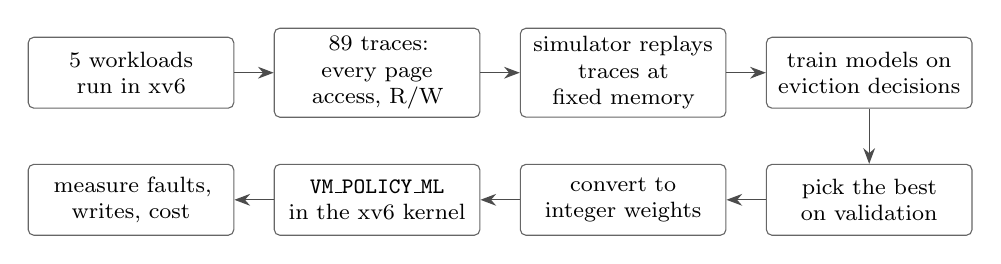
\begin{tikzpicture}[
  box/.style={draw=black!60, rounded corners=2pt, align=center, font=\footnotesize,
              minimum height=9mm, inner sep=3pt, text width=24mm},
  arr/.style={-{Stealth[length=2mm]}, black!70}]
\node[box] (w) {5 workloads\\run in xv6};
\node[box, right=5mm of w] (t) {89 traces:\\every page access, R/W};
\node[box, right=5mm of t] (s) {simulator replays\\traces at fixed memory};
\node[box, right=5mm of s] (m) {train models on\\eviction decisions};
\node[box, below=7mm of m] (v) {pick the best\\on validation};
\node[box, left=5mm of v] (q) {convert to\\integer weights};
\node[box, left=5mm of q] (k) {\code{VM\_POLICY\_ML}\\in the xv6 kernel};
\node[box, left=5mm of k] (r) {measure faults,\\writes, cost};
\draw[arr] (w) -- (t); \draw[arr] (t) -- (s); \draw[arr] (s) -- (m);
\draw[arr] (m) -- (v); \draw[arr] (v) -- (q); \draw[arr] (q) -- (k); \draw[arr] (k) -- (r);
\end{tikzpicture}
\caption{The whole pipeline. Sections 1--3 describe the steps; Section 4 the results.}
\label{fig:pipeline}
\end{figure}

\textbf{How we did it} (Figure~\ref{fig:pipeline}):
\begin{itemize}
\item Recorded every page access of five benchmark programs in xv6 (a B-tree,
a key-value store, graph algorithms, a sort, a matrix multiply): 89 traces,
123 million accesses.
\item Replayed the traces in a simulator at 5, 10 and 20\% of each program's
memory, and trained models to predict how soon each page will be used again.
\item Tried 300 combinations of 12 page features (every combination within
each feature group) and five model types (linear, MLP, ranking MLP, GRU,
embedding); chose the best on validation data only, then tested on new runs
and on new program variants.
\item Converted the chosen linear model to integers (xv6 has no floating point)
and measured it in the kernel: 231 runs, 7 policies.
\end{itemize}

\textbf{What we found.}
\begin{itemize}
\item The kernel's own signals are enough. Knowing every memory access helps
almost nothing; the most useful signal is how long a page has gone unused.
\item A simple linear model (a weighted sum of 4--5 signals) is as good as the
neural models, and costs only a few multiply-adds per page.
\item Integer arithmetic loses nothing compared to floats.
\item The simulator predicts the kernel's results closely.
\end{itemize}

\textbf{Final result.} Inside xv6 the learned linear policy causes fewer page
faults than Clock on every benchmark, on runs and variants it never saw, and
up to \val{k-maxw}\% fewer disk writes (Table~\ref{tab:glance}).

\textbf{What it costs, compared with Clock.}
\begin{itemize}
\item \emph{Slower decisions.} The policy scores every page in memory at every
eviction: about \val{fit-base} timer ticks plus \val{fit-slope} per page (1 tick = 0.1\,\textmu s).
Choosing a victim takes \val{us-sort}\,\textmu s with \val{pages-sort} pages in memory and \val{us-btree}\,\textmu s
with \val{pages-btree} pages: \val{xclock-min}--\val{xclock-max} times Clock, which usually checks only a
few pages, and \val{xaging-min}--\val{xaging-max} times xv6's Aging policy.
\item \emph{More memory.} 33 bytes of bookkeeping per physical page (about
1\,MB for xv6's 32,768 pages, under 1\% of its 128\,MB) and 12 bytes per swap
slot (96\,KB).
\item \emph{One model does not fit all.} A single global model loses to Clock
on matmul (\val{k-g-f-matmul-heldout}\% more faults); the best results need a model per program.
\item \emph{Not yet measured:} whether the fewer faults and saved disk reads
outweigh the slower decisions in total program run time.
\end{itemize}

\begin{table}[!htbp]
\centering\small
\begin{tabular}{@{}lccc@{}}
\toprule
& \textbf{Page faults vs Clock} & \textbf{Disk writes vs Clock} & \textbf{Decision time per eviction} \\
\textbf{Benchmark} & test / held-out & test / held-out & ML vs Clock \\
\midrule
btree & \best{$-$17.7\%} / \best{$-$14.6\%} & $+$2.2\% / \best{$-$3.4\%} & 101.2\,\textmu s vs 3.2\,\textmu s \\
graph & \best{$-$38.6\%} / \best{$-$45.9\%} & \best{$-$95.5\%} / \best{$-$86.2\%} & 59.4\,\textmu s vs 5.6\,\textmu s \\
kv & \best{$-$12.9\%} / \best{$-$12.5\%} & \best{$-$31.8\%} / \best{$-$12.5\%} & 27.5\,\textmu s vs 2.8\,\textmu s \\
matmul & -- / \best{$-$2.7\%} & -- / \best{$-$96.5\%} & 9.2\,\textmu s vs 3.8\,\textmu s \\
sort & \best{$-$4.0\%} / \best{$-$6.7\%} & \best{$-$5.6\%} / \best{$-$7.5\%} & 8.8\,\textmu s vs 3.5\,\textmu s \\
\bottomrule
\end{tabular}

\caption{Results at a glance: the per-workload \textbf{linear} model running
inside xv6 at 10\% memory, compared with Clock on the same runs. Test: new
runs of a known program; held-out: program variants never seen in training
(matmul has held-out traces only). Decision time: test traces (matmul:
held-out), 10\,MHz kernel timer.}
\label{tab:glance}
\end{table}


% ===================================================================
\section{Traces and benchmarks}

\subsection{The benchmarks}

We use five programs that run natively in xv6 (\code{user/*bench.c}); a sixth, \code{lzwbench}, exists but is not used (Table~\ref{tab:bench}). Real
applications such as Redis or SQLite cannot run on xv6 (no network, no
floating point, small files), so each benchmark reproduces the
\emph{memory-access pattern} of a real kind of program. Each one was built so
that no single simple rule (``evict the oldest'', ``evict the least
used'') is best for it; otherwise there would be nothing to learn.

\begin{table}[!htbp]
\centering\small
\begin{tabularx}{\linewidth}{@{}l>{\raggedright\arraybackslash}X>{\raggedright\arraybackslash}X@{}}
\toprule
\textbf{Benchmark} & \textbf{What it does} & \textbf{Why it is hard for one fixed rule} \\
\midrule
\code{btreebench} & A B+tree with one node per 4\,KB page, like a database's page store: inserts, lookups, range scans, a mix, optionally with a write-ahead log. & Lookups reuse the same top nodes (frequency matters), inserts touch new leaves once (recency matters), scans walk leaves in order. \\
\code{kvbench} & A hash table with popular and unpopular keys (Zipf), like a key-value store; read/write mixes A, B, C, D, F as in the YCSB benchmark. & The set of popular keys changes over time, so formerly hot pages must be let go. \\
\code{graphbench} & Breadth-first search and PageRank over a synthetic graph with a few very connected ``hub'' vertices. & BFS order depends on the data; PageRank revisits the hubs every iteration. \\
\code{sortbench} & Merge sort over an array larger than memory. & Mostly sequential; little room to beat simple rules. Used as a sanity check. \\
\code{matmulbench} & Integer matrix multiplication, naive and blocked. & Tiny working sets; the two orders have very different locality. \\
\midrule
\code{lzwbench}$^\ast$ & LZW compression of a real English text (the GPLv3 licence). & Dictionary lookups follow the input text: some entries are reused constantly, most are used once. \\
\bottomrule
\end{tabularx}
\caption{The benchmarks. $^\ast$\code{lzwbench} is implemented but \textbf{not used} in this study (no training, validation, test or kernel runs): its trace (about 109\,MB) is larger than the largest file xv6 can store (about 67\,MB), so it cannot be recorded completely.}
\label{tab:bench}
\end{table}

Each benchmark has several \emph{variants} (different parameters, for example
key-value mode A vs.\ F, or B-tree lookups vs.\ scans) and is run with
several random \emph{seeds}. In total there are 25 variants and 89 traces
(Table~\ref{tab:variants} in the appendix lists them).

\subsection{How a trace is recorded}

Every benchmark reads and writes its data through one small accessor
function. When tracing is on, that function also records one line per access:
\code{R <page>} for a read or \code{W <page>} for a write. The result is the
\emph{complete} sequence of page accesses, not only the page faults. This is
necessary because the best possible eviction choice (Belady's algorithm,
below) needs to know when each page is used next, including uses that hit in
memory.

The trace is written to a file inside xv6 and copied to the host afterwards.
A trace does not depend on how much memory the program is given, so each
trace is recorded once with plenty of memory, and the memory size is chosen
later in simulation.

Each trace was checked before use: the run had to pass, the file had to have
exactly the number of lines and bytes the program reported, a repeated run of
the same seed had to produce a byte-identical trace (22 repeats, all
identical), and replaying the trace under FIFO had to reproduce the kernel's own
eviction count.

\subsection{The dataset}

Each trace is stored with, for every access, the page, whether it was a
write, and the distance to the next access of the same page (the label used
for training, Section~2). The 89 traces hold 123 million accesses.

% ===================================================================
\section{Models and features}

\subsection{What a model does}

At every eviction, the policy looks at all pages currently in memory (the
\emph{candidates}), gives each a score, and evicts the page with the highest
score. A model is trained to predict, for each candidate, how far in the
future that page will be used next (as $\log(1+\text{distance})$, in
accesses). Evicting the page used furthest in the future is exactly what the
optimal policy, Belady's, does; the model tries to imitate it with the
information it has.

\subsection{Features: what the model is allowed to know}

A kernel does not see individual memory accesses: the hardware handles them.
It only sees page faults, and two bits per page that the hardware sets: the
\emph{accessed} bit (the page was used) and the \emph{dirty} bit (it was
written). The kernel can read and clear these bits whenever it scans memory,
which it does at each eviction. We therefore define features in three tiers
(Table~\ref{tab:features}).

\begin{table}[!htbp]
\centering\small
\begin{tabularx}{\linewidth}{@{}lll>{\raggedright\arraybackslash}X@{}}
\toprule
\textbf{Tier} & \textbf{Feature} & \textbf{Meaning} & \textbf{Why it is included} \\
\midrule
\textbf{F} (oracle) & \code{rec} & accesses since the page's last use & classic recency (what LRU uses) \\
 & \code{freq} & number of uses so far & classic frequency (what LFU uses) \\
 & \code{sd} & distinct pages used since its last use & stack distance \\
 & \code{wr} & share of its uses that were writes & write-heavy pages cost a disk write \\
\midrule
\textbf{K} (kernel) & \code{ref} & accessed bit at this scan & what Clock uses \\
 & \code{aging} & 8-bit history of accessed bits & what xv6's Aging uses \\
 & \code{sfreq} & scans that found it accessed & kernel version of frequency \\
 & \code{idle} & scans since it was last found accessed & kernel version of recency \\
 & \code{age} & scans since it was loaded & how new the page is \\
 & \code{dirty} & dirty bit & evicting a dirty page costs a disk write \\
\midrule
\textbf{K+} (refault) & \code{refaults} & times it was evicted and came back & a page that keeps returning is needed \\
 & \code{rdist} & evictions between its last eviction and its return & Linux already measures this (``refault distance'') \\
\bottomrule
\end{tabularx}
\caption{The twelve features. Tier F needs every access, so no kernel can
compute it; it is used only to measure how much a kernel loses by not
seeing accesses. Tiers K and K+ are what a deployable policy can use. A
\emph{refault} is a page fault on a page that was evicted earlier. Counts
enter as $\log(1+\text{count})$.}
\label{tab:features}
\end{table}

\subsection{Model types}

\begin{table}[!htbp]
\centering\small
\begin{tabularx}{\linewidth}{@{}l>{\raggedright\arraybackslash}X>{\raggedright\arraybackslash}X@{}}
\toprule
\textbf{Model} & \textbf{What it is} & \textbf{Why it was tried} \\
\midrule
Linear & a weighted sum of the chosen features & cheap enough for a kernel: a few multiply-adds per page \\
MLP & small neural network, 2 layers of 32 & tests whether non-linear combinations help \\
Ranking loss & linear or MLP trained to put the highest score on Belady's choice within each decision & trains directly on the decision rather than on distances \\
GRU & recurrent network over a page's last 8 gaps between uses & tests whether a page's access rhythm helps \\
Embedding & a learned vector per page plus the last 16 pages used by the program & tests whether knowing which pages are used together helps \\
\bottomrule
\end{tabularx}
\caption{Model types, from cheapest to most expensive.}
\label{tab:models}
\end{table}

Each model is trained either \emph{per workload} or \emph{globally}. A
per-workload model is trained on the training traces of one benchmark, across
all its variants except the held-out one (the btree model learns from insert,
lookup, mixed and mixedwal, and is also tested on the unseen scan variant). A
global model is trained on all five benchmarks together. The global model is the
realistic case for a kernel that does not know which program is running.

\subsection{From a trained model to a kernel policy}

xv6 has no floating point, so the chosen linear models are converted to
integers (\code{tools/ml2/export\_kernel.py}):

\begin{itemize}
\item Each feature is computed as a fixed-point number, the real value times
256. The $\log(1+x)$ is read from a 256-entry table, with a second table for
large values (\code{kernel/mlfeat.h}).
\item Each trained weight is divided by its feature's training standard
deviation, multiplied by 256 and rounded to an integer. The mean and the
constant term are the same for every candidate, so they do not affect which
page has the highest score and are dropped.
\item The score of a page is $\sum_j q_j X_j$: one integer multiply-add per
feature.
\end{itemize}

The policy, \code{VM\_POLICY\_ML}, is the function \code{choose\_ml()} in
\code{kernel/vmpage.c}. At each eviction it scans every candidate (reads and
clears its accessed bit, updates its counters), scores it, and evicts the
highest score. Two rules complete it:

\begin{itemize}
\item \textbf{Probation.} A page loaded fewer than $p$ scans ago is not evicted
while an older candidate exists ($p$ is 0--4, chosen per model on
validation). A brand-new page has no history yet, so its score is least
reliable; this is the same idea as Clock's second chance.
\item \textbf{Ties} go to the page loaded earliest.
\end{itemize}

The refault features need a little memory per swap slot: when a page is
written to swap, the kernel stores the current scan count and the page's
refault count with the slot, and reads them back when the page returns.
Weights are per process: \code{vmctl(VM\_SET\_ML\_WEIGHTS)} loads a model, and
child processes inherit it. The default is the global model. The program
\code{vmrun} runs any command under any policy and model, for example
\code{vmrun ml kv kvbench \ldots}.

As an example, the selected graph model is
$159\cdot\text{idle} - 347\cdot\text{dirty} - 2\cdot\text{sfreq} + 24\cdot\text{rdist}$
(probation 4 scans): evict pages that have been idle longest, and strongly
prefer to keep dirty pages, which would cost a disk write.

% ===================================================================
\section{Training, validation and evaluation}

\subsection{Train / validation / test / held-out split}

The split is fixed before any experiment, so every result is reported on the
same data:

\begin{itemize}
\item \textbf{Held-out} (18 traces): five whole \emph{variants} never seen in
training (\code{kv-F}, \code{btree-scan}, \code{graph-bfs2000},
\code{sort-n60000}, \code{matmul-*128}). This tests a new kind of behaviour.
\item In every other variant, the last seed is \textbf{test} (15 traces), the
second-to-last is \textbf{validation} (15), and the rest are \textbf{train}
(41). Test checks a new run of a familiar behaviour.
\end{itemize}

Models are trained on train, chosen on validation, and reported on test and
held-out, which are never used for any choice. (matmul has one trace per
variant, so its models are chosen on its training traces.)

\subsection{Simulator}

Training and most evaluation use a simulator (\code{tools/ml2/pagesim.c}). It
replays a trace with a fixed number of memory frames and counts page faults,
evictions and disk writes. It implements every xv6 policy (FIFO, Clock,
Aging, LFU), LRU, and Belady's optimal policy. It was checked against
independent code and against the kernel: FIFO, LRU and Belady agree exactly
on all 534 trace $\times$ memory-size cases, and Clock, Aging and LFU match a
direct copy of the kernel's logic.

Memory sizes are 5\%, 10\% and 20\% of the pages each trace touches, which
gives low to high memory pressure.

\subsection{Training data}

A model is used at eviction time, so it is trained on eviction decisions.
Each training trace is replayed under LRU at the three memory sizes. At a
random sample of evictions, up to 32 resident pages are recorded with all
twelve features and their true next-use distance: always Belady's choice,
always the 4 most recently used pages (so the model sees pages that must be
kept), and the rest at random. This gives 4.73 million rows from 357,000
decisions.

Linear models are fitted in closed form (weighted ridge regression). Neural
models use Adam with early stopping on the validation loss.

\subsection{Choosing models}

For linear models, every combination of features was tried: 15 subsets of
the oracle features, 255 subsets of the kernel features, and 30 mixed sets,
each as a per-workload and a global model. That is 28,800 complete replays.
For each tier, the five best subsets on validation were tried with probation
0, 1, 2 and 4, and the best combination on validation at all three memory
sizes was kept. Only then were test and held-out replayed.

\subsection{How performance is measured}

\begin{itemize}
\item \textbf{Faults relative to Clock}: faults of the policy divided by
Clock's faults on the same trace and memory size. Below 1 is better than
Clock. Clock is the baseline because it is the best policy xv6 has. Values
are averaged (geometric mean) over traces.
\item \textbf{Page writes relative to Clock}: the same for disk writes.
\item \textbf{Inside the kernel}: every test and held-out trace was run in
xv6 itself (QEMU, one CPU) at 10\% memory under seven policies, 231 runs in
total. These numbers are the kernel's own counters. The kernel also counts the
time spent choosing each victim (in ticks of its 10\,MHz timer).
\end{itemize}

% ===================================================================
\section{Results}

\subsection{How much room is there?}

\begin{figure}[!htbp]
\centering
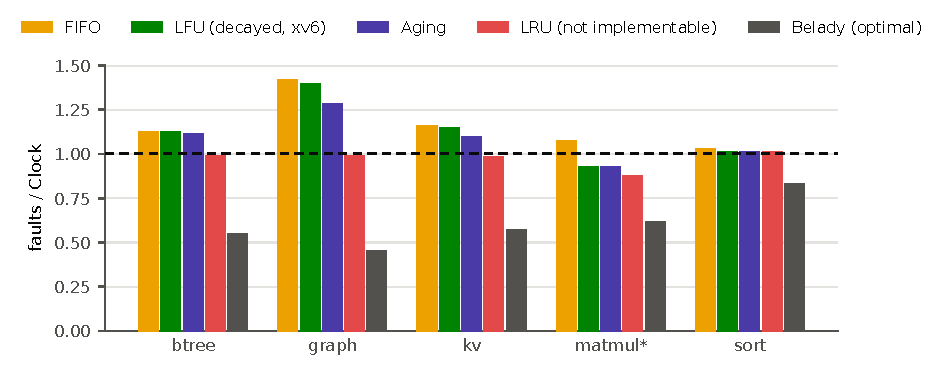
\includegraphics[width=\linewidth]{figs/classical.pdf}
\caption{The policies a kernel has today. Each bar is a policy's faults
divided by Clock's on the same traces (test traces, *matmul: held-out;
averaged over 5/10/20\% memory). The dashed line is Clock: above it is worse,
below it is better. The dark bar is Belady, the best possible, so the gap
between the line and the dark bar is the room for a better policy.}
\label{fig:classical}
\end{figure}

Clock is as good as true LRU on four of the five workloads
(Figure~\ref{fig:classical}). xv6's Aging is only slightly better than FIFO, and its LFU is no better.
The optimum needs \val{b-kv}\%--\val{b-graph}\% fewer faults than Clock on btree, kv and graph, so
there is a lot of room for a better policy there. On sort the room is small
(\val{b-sort}\%).

\subsection{Which signals matter}

\begin{figure}[!htbp]
\centering
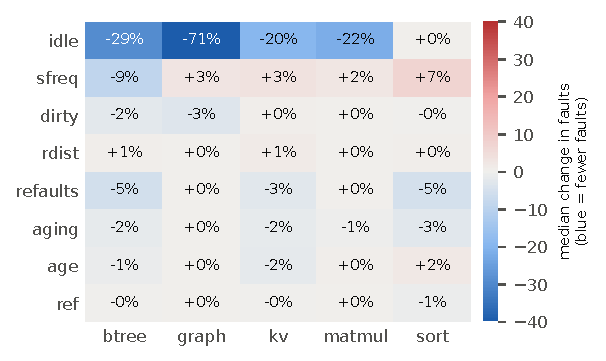
\includegraphics[width=.6\linewidth]{figs/features.pdf}
\caption{What each kernel feature adds: the median change in faults when the
feature is added to a feature set that does not have it, over all such pairs
of sets (per-workload models; test, matmul held-out).}
\label{fig:features}
\end{figure}

\code{idle}, the number of scans since a page was last found in use, is by
far the most useful kernel signal (Figure~\ref{fig:features}): adding it
cuts faults by a median \val{idle-graph}\% on graph, \val{idle-btree}\% on btree, \val{idle-kv}\% on kv and
\val{idle-matmul}\% on matmul. It is the kernel's version of recency, and it is also what Linux's
newest reclaim code (MGLRU) tracks. The other features add a little each, and
which ones help depends on the workload.

The choice of features matters a great deal. Each of the 8 kernel features
(K and K+) is either used or not, which gives $2^8-1 = 255$ non-empty feature
sets. Of these,
more than half are worse than Clock on kv and sort, and up to 126 are more
than three times worse than Clock on graph. Selecting on validation is part
of the method.

\subsection{Kernel signals are enough}

From here on, ``the model'' and ``ML'' mean the selected \emph{linear}
model; Section~4.4 compares the other model types.


\begin{figure}[!htbp]
\centering
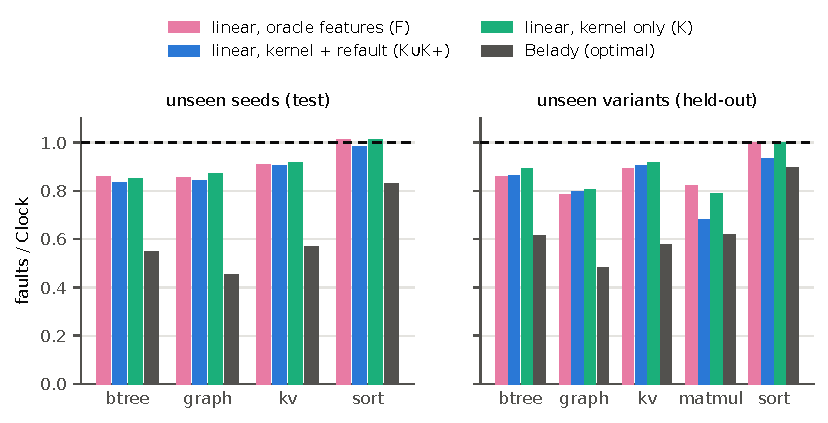
\includegraphics[width=\linewidth]{figs/tiers.pdf}
\caption{The best \textbf{linear} model of each feature tier, chosen on
validation, relative to Clock (averaged over 5/10/20\% memory). Lower is
better.}
\label{fig:tiers}
\end{figure}

\begin{table}[!htbp]
\centering\small
\begin{tabular}{@{}lrrrrr@{}}
\toprule
& \multicolumn{2}{c}{\textbf{per-workload model}} & \multicolumn{2}{c}{\textbf{one global model}} & \textbf{optimum} \\
\cmidrule(lr){2-3}\cmidrule(lr){4-5}
\textbf{Workload} & test & held-out & test & held-out & Belady (test) \\
\midrule
btree & \best{0.833} & \best{0.863} & 0.864 & 0.898 & 0.550 \\
graph & \best{0.845} & \best{0.798} & 0.874 & 0.792 & 0.456 \\
kv & \best{0.905} & \best{0.905} & 0.908 & 0.901 & 0.571 \\
matmul & -- & \best{0.681} & -- & 0.967 & 0.617$^\dagger$ \\
sort & \best{0.983} & \best{0.933} & 1.005 & 0.966 & 0.830 \\
\bottomrule
\end{tabular}

\caption{The selected \textbf{linear} model on kernel+refault (K$\cup$K+)
features, in simulation: faults relative to Clock, averaged over 5/10/20\%
memory. ``Per-workload'': each benchmark's own linear model; ``one global
model'': a single linear model trained on all benchmarks. $^\dagger$held-out.}
\label{tab:headline}
\end{table}

Using only what a kernel can see, the selected model beats Clock on every
workload, on new seeds and on new variants (Table~\ref{tab:headline}), with fewer faults
(test / held-out) on btree \val{s-f-btree-test}\% / \val{s-f-btree-heldout}\%, graph \val{s-f-graph-test}\% / \val{s-f-graph-heldout}\%, kv
\val{s-f-kv-test}\% / \val{s-f-kv-heldout}\%, sort \val{s-f-sort-test}\% / \val{s-f-sort-heldout}\% and matmul \val{s-f-matmul-heldout}\% (held-out). It also makes far fewer disk writes. Evicting a modified
(dirty) page means writing it to disk first; an unmodified page can simply be
dropped. The model sees the dirty bit and prefers unmodified pages, so on graph
it makes \val{s-w-graph-test}\% fewer writes than Clock on test traces and \val{s-w-graph-heldout}\% fewer on
held-out.

Knowing every access does not help much (Figure~\ref{fig:tiers}): on btree, graph and
kv the best oracle model is between \val{orc-better}\% better and \val{orc-worse}\% worse than the kernel
model, and it is worse on matmul and sort. The refault features are worth having: adding them
improves the kernel-only model in all nine workload/split cases.

One global model keeps most of the gain on btree, graph and kv, but little on
matmul (\val{s-g-r-matmul-heldout} vs.\ \val{s-r-matmul-heldout} of Clock's faults).

The gain depends on memory pressure. On graph (test) the model needs \val{s-r-graph-0.1} of
Clock's faults at 10\% memory, but \val{s-r-graph-0.05} at 5\% and \val{s-r-graph-0.2} at 20\%.

\subsection{Bigger models do not pay}

\begin{figure}[!htbp]
\centering
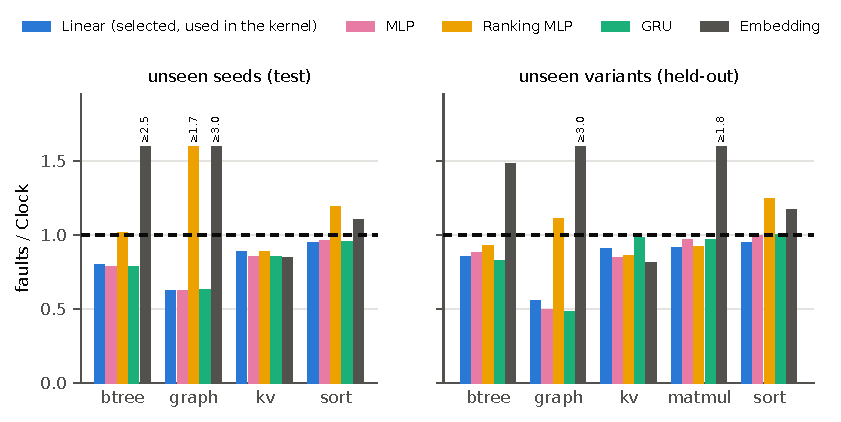
\includegraphics[width=\linewidth]{figs/models.pdf}
\caption{The five model types compared: faults relative to Clock (dashed
line), each benchmark's own model, 10\% memory. Bars that would go off the
chart are cut at 1.6 and labelled with their value ($\geq$: the run was
stopped once it reached that many times Clock's faults).}
\label{fig:models}
\end{figure}


\begin{table}[!htbp]
\centering\small
\begin{tabular}{@{}lrrrrr@{}}
\toprule
\textbf{Workload} & \textbf{Linear} (selected) & \textbf{MLP} & \textbf{Ranking MLP} & \textbf{GRU} & \textbf{Embedding} \\
\midrule
btree & 0.803 & 0.786 & 1.014 & 0.784 & $\geq$2.456 \\
graph & 0.624 & 0.622 & $\geq$1.699 & 0.632 & $\geq$3.000 \\
kv & 0.890 & 0.852 & 0.887 & 0.854 & 0.847 \\
sort & 0.950 & 0.965 & 1.192 & 0.957 & 1.103 \\
\bottomrule
\end{tabular}

\caption{Model types compared: faults divided by Clock's (below 1 is better),
per-workload models, test traces, 10\% memory. Each column is a different model type, each trained
per workload. \emph{Linear (selected)} is the linear model with the feature set
and probation chosen on validation, the one used in Table~\ref{tab:headline}
and in the kernel. MLP
and ranking MLP use the K$\cup$K+ features; GRU and embedding use access
history. $\geq$: the run was stopped once it reached 3$\times$ Clock's
faults.}
\label{tab:nn}
\end{table}

The neural models are not clearly better than the linear one
(Figure~\ref{fig:models}, Table~\ref{tab:nn}). An MLP is somewhat better on kv (\val{mlp-kv-test} vs.\ \val{lin-kv-test} of Clock's
faults), btree (\val{mlp-btree-test} vs.\ \val{lin-btree-test}) and held-out graph (\val{mlp-graph-heldout} vs.\ \val{lin-graph-heldout}), and
worse on sort. Training on the ranking of each decision is worse. The embedding model,
which looks at which pages the whole program used recently, is among the best
on kv but fails badly on btree and graph. A linear score is therefore
the right choice for a kernel: it is as good and costs a few multiply-adds per
page.

\textbf{Integers lose nothing.} With 8-bit integer weights and fixed-point
features, every selected model's result is within $\pm$\val{q8-maxdiff} of the float
version; with 4-bit weights, within \val{q4-maxrel}\% (Table~\ref{tab:quant} in the
appendix).

\subsection{Inside the xv6 kernel}

\begin{figure}[!htbp]
\centering
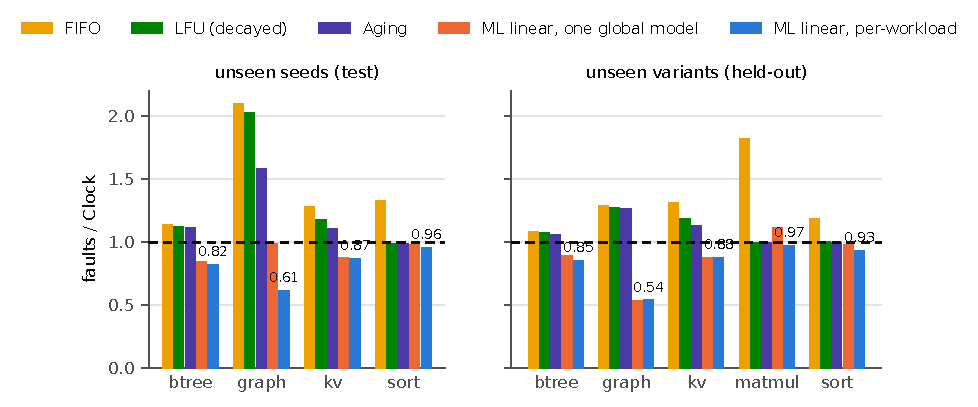
\includegraphics[width=\linewidth]{figs/kernel_faults.pdf}
\caption{Measured in xv6: page faults relative to Clock (dashed line) at
10\% memory, kernel counters, 231 runs. ``ML'' is the selected \textbf{linear}
model with integer weights (the only model type run in the kernel): blue is
each benchmark's own model, orange the single global model. Numbers: the blue
bars.}
\label{fig:kfaults}
\end{figure}

\begin{figure}[!htbp]
\centering
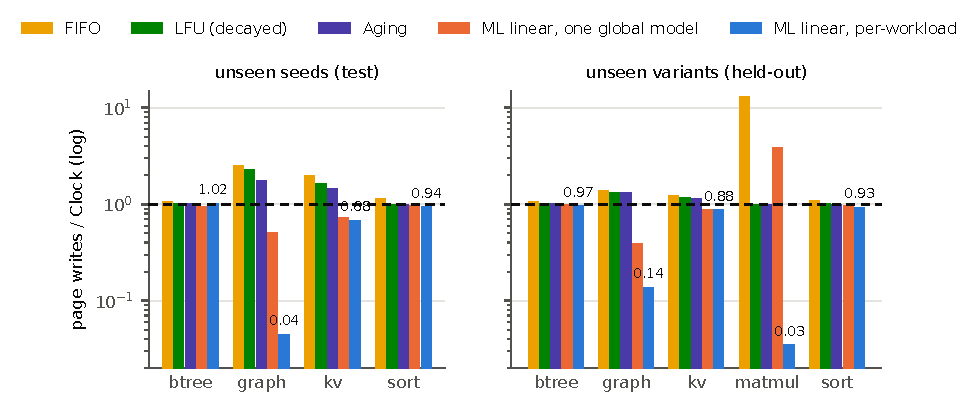
\includegraphics[width=\linewidth]{figs/kernel_writes.pdf}
\caption{Measured in xv6: disk page writes relative to Clock (log scale).}
\label{fig:kwrites}
\end{figure}

\begin{table}[!htbp]
\centering\small
\begin{tabular}{@{}lrrrrrr@{}}
\toprule
& \multicolumn{2}{c}{\textbf{faults / Clock}} & \multicolumn{2}{c}{\textbf{writes / Clock}} & \multicolumn{2}{c}{\textbf{global model, faults}} \\
\cmidrule(lr){2-3}\cmidrule(lr){4-5}\cmidrule(lr){6-7}
\textbf{Workload} & test & held-out & test & held-out & test & held-out \\
\midrule
btree & \best{0.823} & \best{0.854} & 1.022 & \best{0.966} & 0.843 & 0.893 \\
graph & \best{0.614} & \best{0.541} & \best{0.045} & \best{0.138} & 0.989 & 0.535 \\
kv & \best{0.871} & \best{0.875} & \best{0.682} & \best{0.875} & 0.875 & 0.878 \\
matmul & -- & \best{0.973} & -- & \best{0.035} & -- & 1.115 \\
sort & \best{0.960} & \best{0.933} & \best{0.944} & \best{0.925} & 0.980 & 0.977 \\
\bottomrule
\end{tabular}

\caption{\code{VM\_POLICY\_ML} (the selected \textbf{linear} models, integer
weights) measured in xv6 at 10\% memory, relative to Clock. First four columns:
each benchmark's own model; last two: the single global model.}
\label{tab:kernel}
\end{table}

Inside the kernel the learned policy beats Clock on every workload, on new
seeds and new variants (Figure~\ref{fig:kfaults}, Table~\ref{tab:kernel}):
fewer faults (test / held-out) on btree \val{k-f-btree-test}\% / \val{k-f-btree-heldout}\%, graph
\val{k-f-graph-test}\% / \val{k-f-graph-heldout}\%, kv \val{k-f-kv-test}\% / \val{k-f-kv-heldout}\%, sort \val{k-f-sort-test}\% / \val{k-f-sort-heldout}\% and matmul
\val{k-f-matmul-heldout}\% (held-out). Disk writes drop by \val{k-w-graph-test}\% / \val{k-w-graph-heldout}\% on graph and
\val{k-w-matmul-heldout}\% on matmul (Figure~\ref{fig:kwrites}). The global model beats Clock
everywhere except matmul (\val{k-g-f-matmul-heldout}\% more faults).

\begin{figure}[!htbp]
\centering
\begin{minipage}[c]{.40\linewidth}
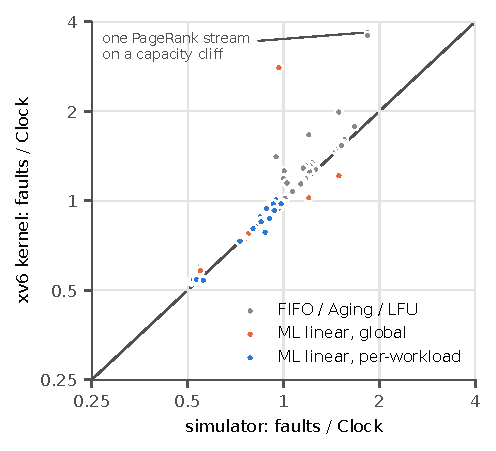
\includegraphics[width=\linewidth]{figs/kernel_vs_sim.pdf}
\end{minipage}\hfill
\begin{minipage}[c]{.56\linewidth}
\caption{Each dot is one trace and policy: the simulator's prediction ($x$)
against the kernel's measurement ($y$), both relative to Clock. Dots on the
diagonal mean the simulator predicted the kernel exactly. The outlier is one
PageRank trace that sits at a memory size where two more frames halve the
faults; the kernel effectively has about two more frames for it than the
simulator.}
\label{fig:kvs}
\end{minipage}
\end{figure}

The simulator predicted the kernel well (Figure~\ref{fig:kvs}): for the ML
models, Clock, Aging and LFU the median ratio of kernel to simulated faults
is between \val{kvs-min} and \val{kvs-max} on every workload (the global model on matmul
does better in the kernel, \val{kvs-gmatmul}). So the simulation results of
Sections 4.1--4.4 carry over to the real kernel. FIFO does worse in the kernel than simulated, most likely because there it
also evicts the program's own code and stack pages, which the traces do not
include.

\begin{table}[!htbp]
\centering\small
\begin{tabular}{@{}llrrrrrr@{}}
\toprule
& & \textbf{pages in} & \multicolumn{4}{c}{\textbf{timer ticks per eviction}} & \textbf{ML time} \\
\cmidrule(lr){4-7}
\textbf{Workload} & \textbf{Split} & \textbf{memory} & Clock & Aging & ML global & ML per-wl. & \textbf{per eviction} \\
\midrule
btree & test & 249 & 31.7 & 411.7 & 896.6 & 1011.6 & 101.2\,\textmu s \\
btree & held-out & 222 & 30.2 & 410.3 & 872.3 & 978.9 & 97.9\,\textmu s \\
graph & test & 160 & 55.6 & 277.0 & 543.4 & 594.4 & 59.4\,\textmu s \\
graph & held-out & 170 & 37.8 & 288.7 & 616.6 & 639.1 & 63.9\,\textmu s \\
kv & test & 62 & 28.0 & 130.0 & 250.8 & 275.2 & 27.5\,\textmu s \\
kv & held-out & 56 & 29.7 & 124.5 & 245.4 & 265.1 & 26.5\,\textmu s \\
matmul & held-out & 9 & 38.1 & 45.9 & 83.3 & 92.5 & 9.2\,\textmu s \\
sort & test & 10 & 35.1 & 48.4 & 82.2 & 88.1 & 8.8\,\textmu s \\
sort & held-out & 16 & 31.9 & 60.2 & 108.8 & 120.5 & 12.1\,\textmu s \\
\bottomrule
\end{tabular}

\caption{Time to choose a victim in xv6, measured by the kernel's 10\,MHz timer
(1 tick = 0.1\,\textmu s of emulated time), mean per eviction at 10\% memory.
``Pages in memory'' is how many pages the policy had to choose from. Last
column: the per-workload ML model in microseconds.}
\label{tab:cost}
\end{table}

\textbf{The cost.} The learned policy scores every page in memory at every
eviction, so its decision time grows with the number of pages: about
\val{fit-base} ticks plus \val{fit-slope} per page (Table~\ref{tab:cost}), from \val{us-sort}\,\textmu s on sort (\val{pages-sort}
pages) to \val{us-btree}\,\textmu s on btree (\val{pages-btree} pages). That is \val{xclock-min}--\val{xclock-max} times
Clock and \val{xaging-min}--\val{xaging-max} times Aging, and the main thing to improve.

% ===================================================================
% ===================================================================
\FloatBarrier
\appendix
\section*{Appendix: data and tables}
\addcontentsline{toc}{section}{Appendix}
\renewcommand{\thetable}{A\arabic{table}}
\setcounter{table}{0}

\begin{table}[!htbp]
\centering\small
\begin{tabular}{@{}llrrrl@{}}
\toprule
\textbf{Workload} & \textbf{Variant} & \textbf{Traces} & \textbf{Accesses (mean)} & \textbf{Pages} & \textbf{Split} \\
\midrule
btree & insert, lookup, mixed, mixed+WAL & 5 each & 210K--328K & 1.8K--4.1K & train/val/test \\
 & scan & 5 & 413K & 2.2K & held-out \\
\midrule
graph & BFS+PageRank 1000$\times$3 & 3 & 6.2M & 999 & train/val/test \\
 & BFS+PageRank 2000$\times$1 & 5 & 6.3M & 2.0K & train/val/test \\
 & PageRank 2000$\times$2 & 3 & 6.1M & 1.7K & train/val/test \\
 & BFS 2000 & 3 & 3.2M & 1.7K & held-out \\
\midrule
kv & A, A+rehash, A+value sizes, B, C, D & 5 each & 100K--479K & 527--749 & train/val/test \\
 & F & 5 & 321K & 528 & held-out \\
\midrule
matmul & naive / blocked, n = 64, 96 & 1 each & 528K--2.0M & 12--27 & train \\
 & naive / blocked, n = 128 & 1 each & 4.2M--4.7M & 48 & held-out \\
\midrule
sort & n = 20,000, 40,000 & 3 each & 867K--1.9M & 40--79 & train/val/test \\
 & n = 60,000 & 3 & 2.8M & 118 & held-out \\
\bottomrule
\end{tabular}

\caption{The 89 traces. ``Pages'' is the number of distinct pages a trace
touches; memory sizes are 5/10/20\% of it.}
\label{tab:variants}
\end{table}

\begin{table}[!htbp]
\centering\small
\begin{tabular}{@{}ll@{}}
\toprule
\textbf{Model} & \textbf{Features (probation in scans)} \\
\midrule
btree & aging + idle + age + dirty + refaults (0) \\
graph & sfreq + idle + dirty + rdist (4) \\
kv & aging + idle + dirty + refaults + rdist (2) \\
matmul & aging + idle + dirty + refaults + rdist (0) \\
sort & ref + dirty + refaults + rdist (4) \\
global & idle + dirty + refaults + rdist (4) \\
\bottomrule
\end{tabular}

\caption{The selected kernel+refault models, chosen on validation. These are
the weights the kernel runs.}
\label{tab:chosen}
\end{table}

\begin{table}[!htbp]
\centering\small
\begin{tabular}{@{}llrrrr@{}}
\toprule
\textbf{Workload} & \textbf{Split} & \textbf{float} & \textbf{4-bit} & \textbf{8-bit} & \textbf{12-bit} \\
\midrule
btree & test & 0.833 & 0.834 & 0.833 & 0.833 \\
btree & held-out & 0.863 & 0.875 & 0.862 & 0.863 \\
graph & test & 0.845 & 0.848 & 0.845 & 0.845 \\
graph & held-out & 0.798 & 0.812 & 0.799 & 0.798 \\
kv & test & 0.905 & 0.905 & 0.905 & 0.904 \\
kv & held-out & 0.905 & 0.903 & 0.904 & 0.904 \\
matmul & held-out & 0.681 & 0.681 & 0.681 & 0.681 \\
sort & test & 0.983 & 0.983 & 0.983 & 0.983 \\
sort & held-out & 0.933 & 0.932 & 0.933 & 0.933 \\
\bottomrule
\end{tabular}

\caption{Float vs.\ integer scoring (faults relative to Clock, simulation,
averaged over 5/10/20\% memory).}
\label{tab:quant}
\end{table}

\begin{table}[!htbp]
\centering\small
\begin{tabular}{@{}llrrrrrr@{}}
\toprule
\textbf{Workload} & \textbf{Split} & \textbf{FIFO} & \textbf{Aging} & \textbf{LFU} & \textbf{ML global} & \textbf{ML per-wl.} & \textbf{ML K only} \\
\midrule
btree & test & 1.143 & 1.116 & 1.127 & 0.843 & 0.823 & 0.824 \\
graph & test & 2.096 & 1.585 & 2.027 & 0.989 & 0.614 & 0.630 \\
kv & test & 1.284 & 1.107 & 1.175 & 0.875 & 0.871 & 0.908 \\
sort & test & 1.331 & 0.988 & 0.991 & 0.980 & 0.960 & 0.988 \\
btree & held-out & 1.087 & 1.063 & 1.073 & 0.893 & 0.854 & 0.893 \\
graph & held-out & 1.289 & 1.264 & 1.274 & 0.535 & 0.541 & 0.550 \\
kv & held-out & 1.312 & 1.133 & 1.187 & 0.878 & 0.875 & 0.924 \\
matmul & held-out & 1.820 & 0.999 & 0.999 & 1.115 & 0.973 & 0.999 \\
sort & held-out & 1.190 & 0.998 & 1.006 & 0.977 & 0.933 & 0.998 \\
\bottomrule
\end{tabular}

\caption{All in-kernel results: faults relative to Clock at 10\% memory
(kernel counters, geometric mean over traces).}
\label{tab:kernelall}
\end{table}

\begin{table}[!htbp]
\centering\small
\begin{tabularx}{\linewidth}{@{}l>{\raggedright\arraybackslash}X@{}}
\toprule
\textbf{What} & \textbf{Where} \\
\midrule
Benchmarks & \code{user/btreebench.c}, \code{kvbench.c}, \code{graphbench.c}, \code{sortbench.c}, \code{matmulbench.c} \\
Trace collection & \code{tools/make\_stream\_manifest.py}, \code{run\_stream\_lanes.sh}, \code{check\_streams.py}, \code{stream\_dataset.py} \\
Simulator, training, selection & \code{tools/ml2/} (\code{pagesim.c}, \code{build\_datasets.py}, \code{sweep\_linear.py}, \code{final.py}) \\
Kernel policy & \code{kernel/vmpage.c} (\code{choose\_ml}), \code{kernel/mlfeat.h}, \code{kernel/mlweights.h}, \code{user/vmrun.c} \\
Kernel evaluation & \code{tools/ml2/kernel\_eval.py}, \code{kernel\_vs\_sim.py} \\
All results and models & \code{report/results2/} (every generated table: \code{tables.md}), \code{report/models2/} \\
\bottomrule
\end{tabularx}
\caption{Where everything is.}
\end{table}

\end{document}
